\documentclass[10pt]{beamer}
\usepackage{ragged2e}
\usepackage[utf8]{inputenc}
\usepackage{multicol}
\usepackage[cache=false]{minted}
\usepackage{caption}
\usepackage{subcaption}

\usemintedstyle{solarized-light}
\captionsetup{font=footnotesize,labelfont={bf,sf}}
\captionsetup[sub]{font=scriptsize,labelfont={bf,sf}}
\setlength{\abovecaptionskip}{3pt plus 1pt minus 2pt}
\setlength{\belowcaptionskip}{4pt plus 1pt minus 2pt}
\bibliographystyle{plainurl}
\setbeamertemplate{bibliography item}{\insertbiblabel}

\apptocmd{\frame}{}{\justifying}{}
\usetheme{Montpellier}
\usecolortheme{beaver}
\usefonttheme{structurebold}
\definecolor{links}{HTML}{2986CC}
\hypersetup{colorlinks,linkcolor=,urlcolor=links}
\setbeamertemplate{caption}[numbered]
\setbeamertemplate{footline}[frame number]
\beamertemplatenavigationsymbolsempty
\setbeamercolor{bibliography item}{parent=palette primary}
\setbeamercolor*{bibliography entry title}{parent=palette primary}

\newcommand{\txt}[1]{\mintinline{text}{#1}}

\title{Binary classification of machine failures}
\subtitle{Project work in Machine Learning \& Data Mining}
\author{ Andrea Terenziani \\ \footnotesize \href{mailto:andrea.terenziani@studio.unibo.it}{andrea.terenziani@studio.unibo.it}}
\institute{University of Bologna}
\date{}

\begin{document}

\begin{frame}
\titlepage
\end{frame}

\begin{frame}{\contentsname}
\begin{multicols}{2}
\tableofcontents
\end{multicols}
\end{frame}

\section{INTRODUCTION}
\begin{frame}{\secname}
\end{frame}

\subsection{The project}
\begin{frame}{\subsecname}
This project is based on the Kaggle challenge of the same name \cite{playground-series-s3e17}.

The data consisted in a set of various industrial devices, each described through attributes like torque or operating temperature, that did or did not suffer some kind of failure.

The task was therefore a binary classification between failed (class 1) and not-failed (class 0), which was done through several different models, from decision trees to a support vector machine.

All estimators (except for the first, as will be shown) were first run using default parameters, to achieve a baseline performance, then tuned with cross validation. All this was done using the \txt{scikit-learn} python package \cite{scikit-learn}, with the cross validation being performed using the \txt{GridSearchCV} and \txt{StratifiedKFold} classes.
\end{frame}

\subsection{Overview of the data}

\begin{frame}[label={attributes}]{\subsecname}
The attributes of each device are the following:
\begin{table}
    \centering
    \resizebox{\textwidth}{!}{
        \begin{tabular}{l|c|l}
            \textbf{Attribute} & \textbf{Datatype} & \textbf{Description} \\
            \hline\hline
            id & \txt{Int} & Device identifier  \\
            Product Id & \txt{String} & Unique Id, combination of the Type attribute and a number identifier \\
            Type & \txt{String} & Type of product/device (possible values: "L","M","H") \\       
            Air Temperature & \txt{Float} & Air temperature (Kelvin) \\
            Process Temperature & \txt{Float} & Production process temperature (Kelvin) \\
            Rotational Speed & \txt{Int} & Speed in RPM \\
            Torque & \txt{Float} & Torque in Nm (Newton Meter) \\
            Tool Wear & \txt{Int} & Time unit needed to wear down the product/tool \\
            TWF & \txt{Int} & Tool Wear Failure (binary) \\
            HDF & \txt{Int} & Heat Dissipation Failure (binary) \\
            PWF & \txt{Int} & Power Failure (binary) \\
            OSF & \txt{Int} & Overstrain Failure (binary) \\
            RNF & \txt{Int} & Random Failure (binary) \\
            \textbf{Machine Failure} & \txt{Int} & Failure binary feature (\textit{class attribute})
        \end{tabular}
    }
\end{table}
The fraction of devices belonging to each class is 98.43\% for class 0 and 1.57\% for class 1, a ratio of around 62 to 1.
\end{frame}

\begin{frame}{\subsecname}

\begin{figure}
    \centering
    \begin{subfigure}[c]{0.5\textwidth}
        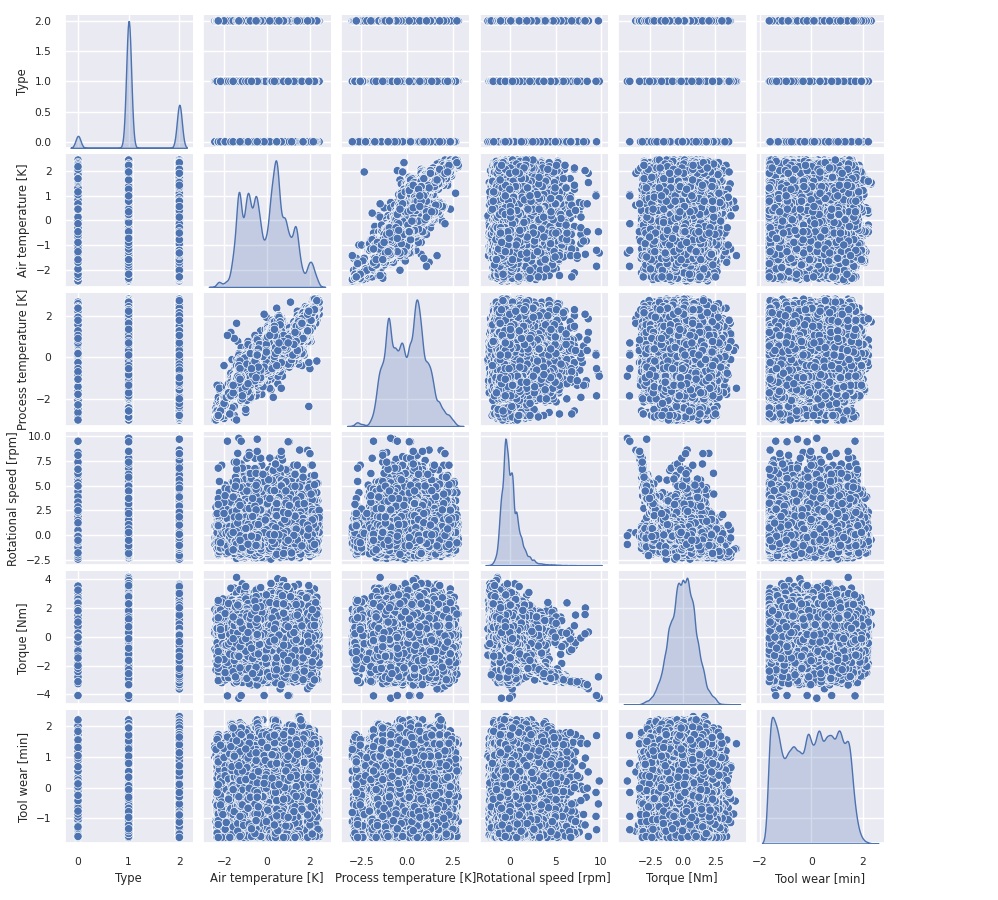
\includegraphics[width=\linewidth]{images/pairplot0.png}
        \caption{Class 0 pairplot}
        \label{fig:pairplot_0}
    \end{subfigure}\hfill
    \begin{subfigure}[c]{0.5\textwidth}
        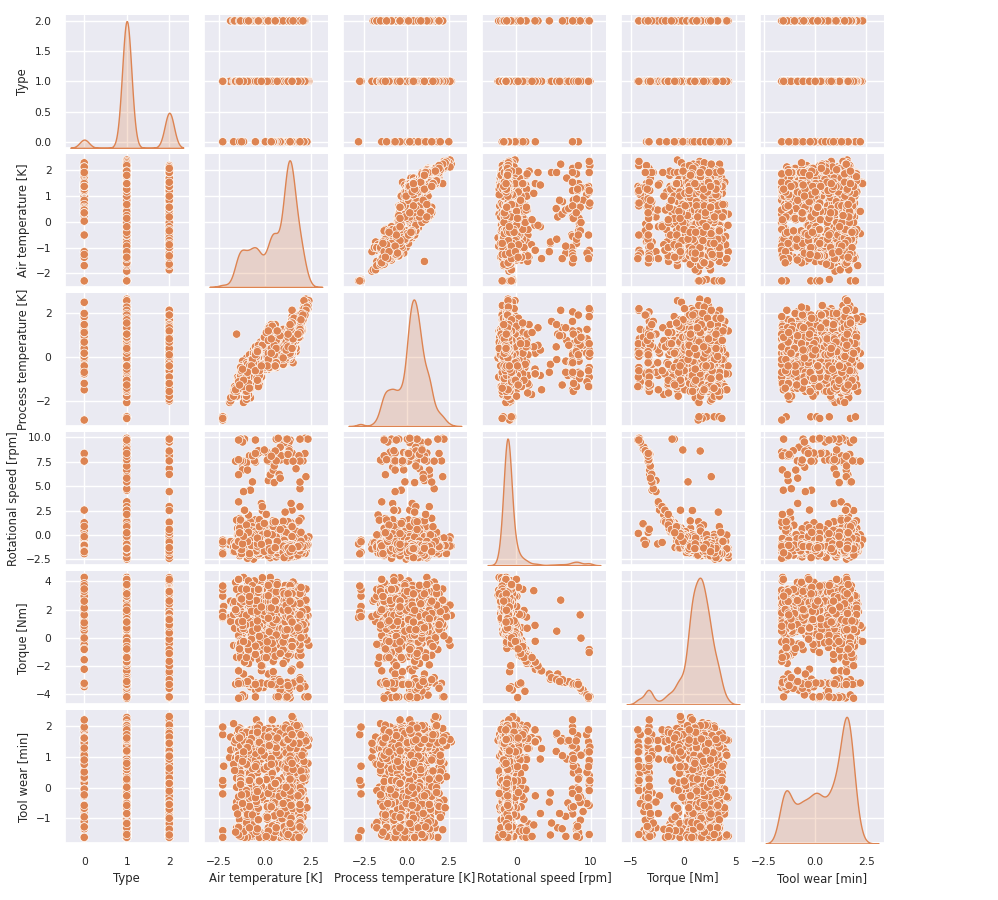
\includegraphics[width=\linewidth]{images/pariplot1.png}
        \caption{Class 1 pairplot}
        \label{fig:pairplot_1}
    \end{subfigure}
    \caption{Feature distributions per class (after preprocessing)}
    \label{fig:pairplots}
\end{figure}
\end{frame}

\subsection{Challenges}
\begin{frame}{\subsecname}
The main issue with the data is its extreme \textit{imbalance} between majority and minority class (see slide \ref{attributes}). This is addressed (mostly) by:
\begin{enumerate}
    \justifying
    \small
    \item resampling the minority class 
    \item choosing an appropriate metric for tuning
\end{enumerate}

Secondly, the dataset was actually generated from another one, leading to a few rows (822 out of around 132k) being clearly invalid and getting removed (their data couldn't be considered "reliable"). Specifically, these had a class inconsistent with their binary failure point (e.g., "Machine Failure" set to 0 but "HDF" set to 1).
\end{frame}

\subsection{Preprocessing and Resampling}
\begin{frame}{\subsecname}
The preprocessing simply comprised:
\begin{itemize}
    \small
    \justifying
    \item Removing the aforementioned incoherent rows, together with the TWF, HDF, PWF, OSF, RNF attributes (which would just be a copy of the class attribute)
    \item Removing the Product ID attribute, not relevant to the classification
    \item Normalizing all remaining features (except for Type, which is categorical)
\end{itemize}

The resampling specifically consisted in \textit{oversampling} the minority class to reach a minority-majority ratio of 1 to 10. This was done using the \mintinline{text}{imbalanced-learn} Python package \cite{imblearn}, which offers an implementation of the SMOTE oversampling method \cite{DBLP:journals/corr/abs-1106-1813}. Undersampling the majority was instead discarded because, in this case, it would mean removing a large number of rows to achieve the same ratio.

\end{frame}

\section{MODELLING}
\begin{frame}{\secname}
\end{frame}

\subsection{Decision Tree}

\begin{frame}{\subsecname\ : Baselines(s)}

The first model tested was a \txt{DecisionTreeClassifier}, which was also used to fine-tune the method used for subsequent estimators. From figure \ref{fig:DT_base_overs}, we see that using the oversampled data already produced a slight improvement.

\begin{figure}
    \centering
    \begin{subfigure}[c]{0.4\textwidth}
        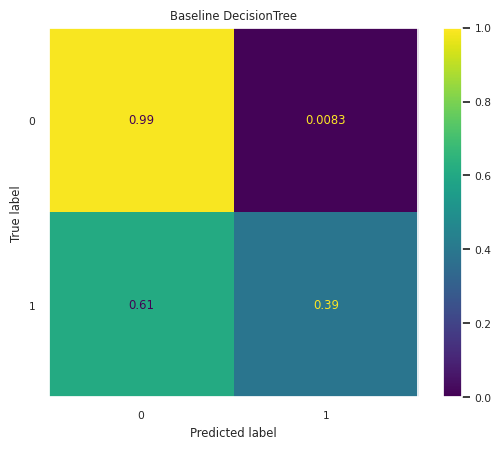
\includegraphics[width=\textwidth]{images/models/DT_base.png}
        \caption{Using the original dataset}
        \label{fig:DT_base}
    \end{subfigure}
    \begin{subfigure}[c]{0.4\textwidth}
        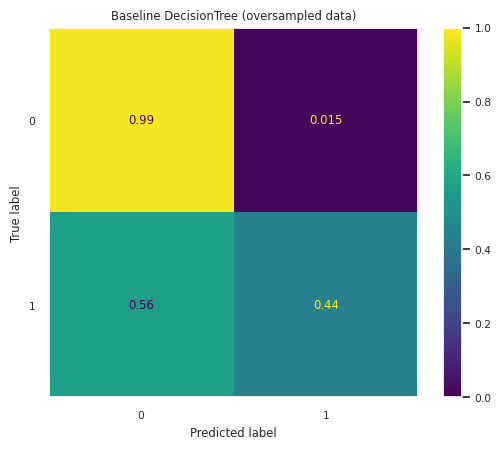
\includegraphics[width=\textwidth]{images/models/DT_base_overs.png}
        \caption{Using oversampled dataset}
        \label{fig:DT_base_overs}
    \end{subfigure}
    \caption{\txt{DecisionTreeClassifier} baselines}
    \label{fig:DT_bases}
\end{figure}
\end{frame}

\begin{frame}{\subsecname\: Grid search}
\begin{columns}[t]
    \column{0.37\textwidth}
    \justifying
    After confirming the choice of using the oversampled data, a grid search for each of the four main scoring metrics shows that the one we should focus on is \txt{recall_macro}, see figure \ref{fig:DT_recmacro}, which will be used for all subsequent tunings.

    This is because it "requires" a model that correctly classifies as many classes as possible, giving more importance to the minority.
    \column{0.63\textwidth}
        \begin{figure}
            \centering
            \vspace{-2.0em} 
            \begin{columns}[t]
                \column{.5\textwidth}
                    \centering
                    \begin{subfigure}[c]{\textwidth}
                        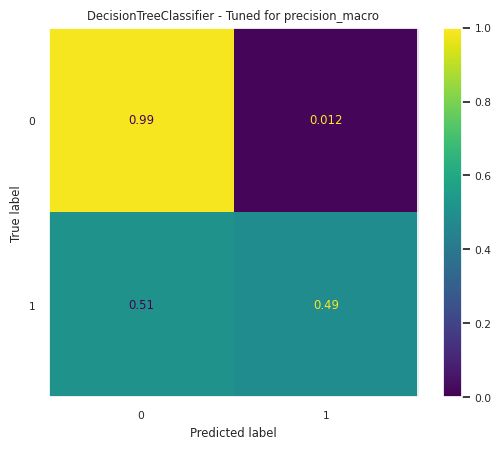
\includegraphics[width=\textwidth]{images/models/DT_precmacro.png}
                        \caption{\txt{precision_macro}}
                        \label{fig:DT_precmacro}
                    \end{subfigure} \\
                    \vspace{-.4em} 
                    \begin{subfigure}[c]{\textwidth}
                        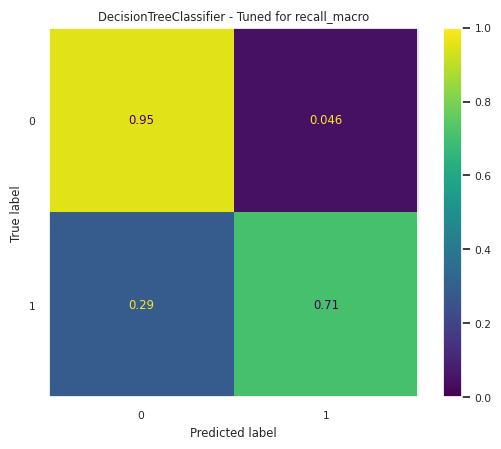
\includegraphics[width=\textwidth]{images/models/DT_recmacro.png}
                        \caption{\txt{recall_macro}}
                        \label{fig:DT_recmacro}
                    \end{subfigure}
                \column{.5\textwidth}
                    \centering
                    \begin{subfigure}[c]{\textwidth}
                        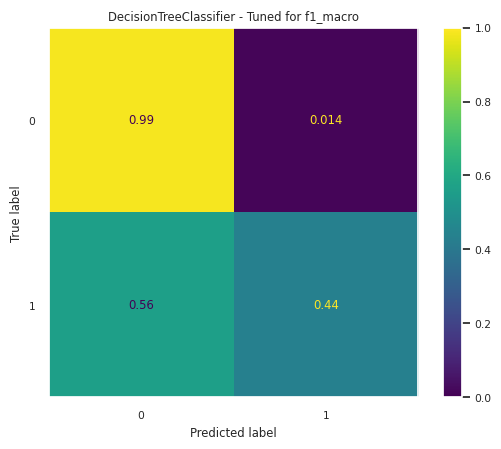
\includegraphics[width=\textwidth]{images/models/DT_f1macro.png}
                        \caption{\txt{f1_macro}}
                        \label{fig:DT_f1macro}
                    \end{subfigure} \\
                    \vspace{-.4em} 
                    \begin{subfigure}[c]{\textwidth}
                        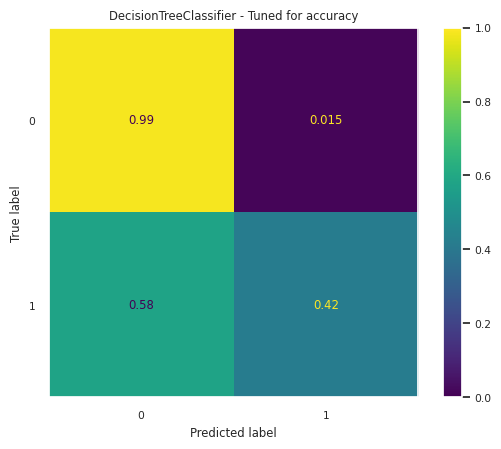
\includegraphics[width=\textwidth]{images/models/DT_acc.png}
                        \caption{\txt{accuracy}}
                        \label{fig:DT_acc}
                    \end{subfigure}
            \end{columns}
            \vspace{-0.8em} 
            %\caption{Tuned results for each metric}
            \label{fig:DT_grids}
        \end{figure}
\end{columns}

\end{frame}

\begin{frame}{\subsecname : Final results}
\begin{columns}
    \column{0.5\textwidth}
    \begin{table}
        \footnotesize
        \centering
        \begin{tabular}{ll}
            parameter & tuned value \\
            \hline\hline
            \txt{max_depth} & 14 \\
            \txt{criterion} & \txt{"gini"} \\
            \txt{class_weight} & \txt{"balanced"} \\
        \end{tabular}
        %\label{tab:my_label}
    \end{table}
    \column{0.5\textwidth}
    \begin{table}
        \footnotesize
        \centering
        \begin{tabular}{lc}
            metric & result \\
            \hline\hline
            \txt{recall} (class 1) & 71\% \\
            \txt{recall_macro} & 83\% \\
        \end{tabular}
        %\label{tab:my_label}
    \end{table}
\end{columns}

\begin{figure}
    \centering
    \begin{subfigure}[c]{0.4\textwidth}
        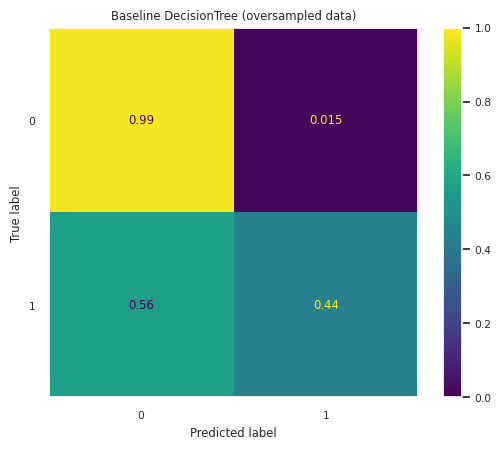
\includegraphics[width=\textwidth]{images/models/DT_base_overs.png}
        \caption{Baseline}
        \label{fig:DT_baseline}
    \end{subfigure}
    \begin{subfigure}[c]{0.4\textwidth}
        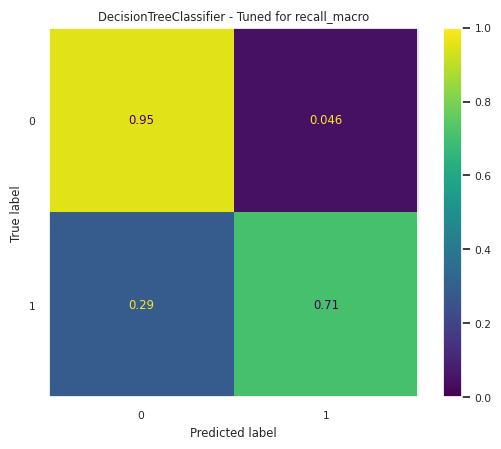
\includegraphics[width=\textwidth]{images/models/DT_recmacro.png}
        \caption{Tuned}
        \label{fig:DT_tuned}
    \end{subfigure}
    \caption{\subsecname\ results}
    \label{fig:DT_results}
\end{figure}
\end{frame}

\subsection{Random Forest}

\begin{frame}{\subsecname}
\begin{columns}
    \column{0.5\textwidth}
    \begin{table}
        \footnotesize
        \centering
        \begin{tabular}{ll}
            parameter & tuned value \\
            \hline\hline
            \txt{max_depth} & 9 \\
            \txt{criterion} & \txt{"gini"} \\
            \txt{class_weight} & \txt{"balanced"} \\
            \txt{n_estimators} & 100
        \end{tabular}
        %\label{tab:my_label}
    \end{table}
    \column{0.5\textwidth}
    \begin{table}
        \footnotesize
        \centering
        \begin{tabular}{lc}
            metric & result \\
            \hline\hline
            \txt{recall} (class 1) & 84\% \\
            \txt{recall_macro} & 89\% \\
        \end{tabular}
        %\label{tab:my_label}
    \end{table}
\end{columns}

\begin{figure}
    \centering
    \begin{subfigure}[c]{0.4\textwidth}
        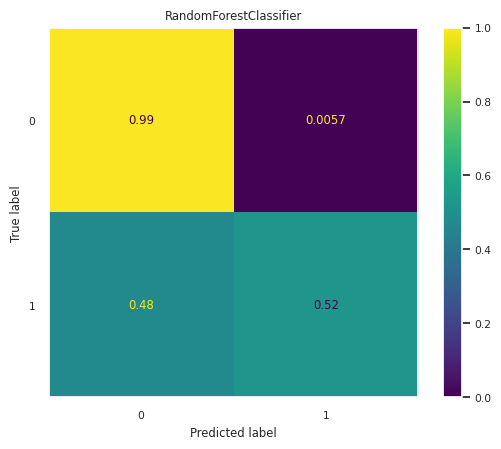
\includegraphics[width=\textwidth]{images/models/RF_base.png}
        \caption{Baseline}
        \label{fig:RF_base}
    \end{subfigure}
    \begin{subfigure}[c]{0.4\textwidth}
        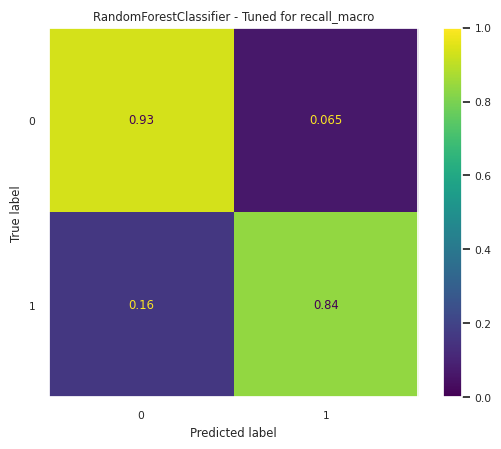
\includegraphics[width=\textwidth]{images/models/RF_tuned.png}
        \caption{Tuned}
        \label{fig:RF_tuned}
    \end{subfigure}
    \caption{\subsecname\ results}
    \label{fig:RF_results}
\end{figure}
\end{frame}

\subsection{AdaBoost}
\begin{frame}{\subsecname}
\begin{columns}
    \column{0.5\textwidth}
    \begin{table}
        \footnotesize
        \centering
        \begin{tabular}{ll}
            parameter & tuned value \\
            \hline\hline
            \txt{learning_rate} & 1.4 \\
            \txt{n_estimators} & 100
        \end{tabular}
        %\label{tab:my_label}
    \end{table}
    \column{0.5\textwidth}
    \begin{table}
        \footnotesize
        \centering
        \begin{tabular}{lc}
            metric & result \\
            \hline\hline
            \txt{recall} (class 1) & 55\% \\
            \txt{recall_macro} & 77\% \\
        \end{tabular}
        %\label{tab:my_label}
    \end{table}
\end{columns}

\begin{figure}
    \centering
    \begin{subfigure}[c]{0.4\textwidth}
        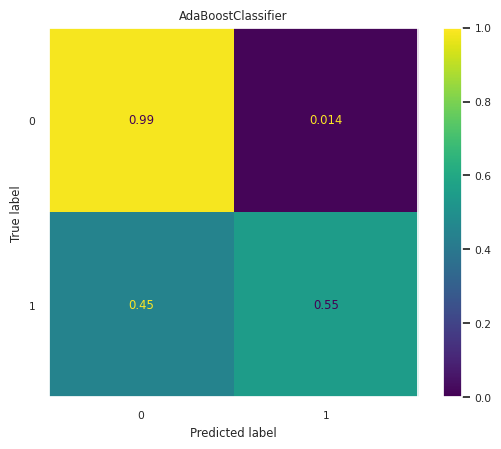
\includegraphics[width=\textwidth]{images/models/Ada_base.png}
        \caption{Baseline}
        %\label{fig:Ada_base}
    \end{subfigure}
    \begin{subfigure}[c]{0.4\textwidth}
        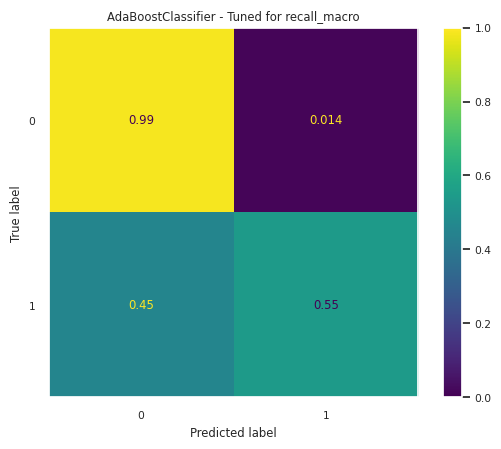
\includegraphics[width=\textwidth]{images/models/Ada_tuned.png}
        \caption{Tuned}
        %\label{fig:Ada_tuned}
    \end{subfigure}
    \caption{\subsecname\ results}
    %\label{fig:Ada_results}
\end{figure}
\end{frame}

\subsection{K-Nearest Neighbor}
\begin{frame}{\subsecname}
\begin{columns}
    \column{0.5\textwidth}
    \begin{table}
        \footnotesize
        \centering
        \begin{tabular}{ll}
            parameter & tuned value \\
            \hline\hline
            \txt{algorithm} & \txt{"kd_tree"} \\
            \txt{metric} & \txt{"manhattan"} \\
            \txt{leaf_size} & 40 \\
            \txt{n_neighbors} & 1 \\
        \end{tabular}
        %\label{tab:my_label}
    \end{table}
    \column{0.5\textwidth}
    \begin{table}
        \footnotesize
        \centering
        \begin{tabular}{lc}
            metric & result \\
            \hline\hline
            \txt{recall} (class 1) & 45\% \\
            \txt{recall_macro} & 72\% \\
        \end{tabular}
        %\label{tab:my_label}
    \end{table}
\end{columns}

\begin{figure}
    \centering
    \begin{subfigure}[c]{0.4\textwidth}
        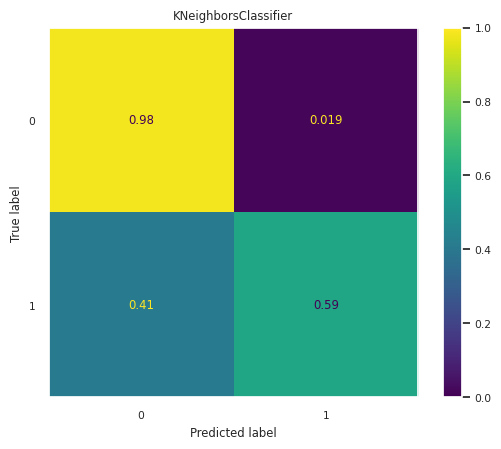
\includegraphics[width=\textwidth]{images/models/KNN_base.png}
        \caption{Baseline}
        %\label{fig:Ada_base}
    \end{subfigure}
    \begin{subfigure}[c]{0.4\textwidth}
        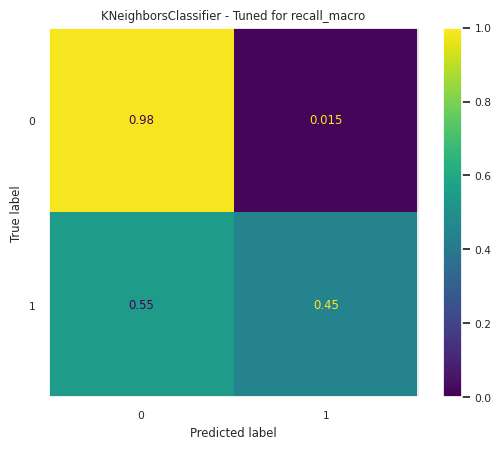
\includegraphics[width=\textwidth]{images/models/KNN_tuned.png}
        \caption{Tuned}
        %\label{fig:Ada_tuned}
    \end{subfigure}
    \caption{\subsecname\ results}
    %\label{fig:Ada_results}
\end{figure}
\end{frame}

\subsection{Gaussian Naive Bayes}
\begin{frame}{\subsecname}
\begin{columns}
    \column{0.5\textwidth}
    \begin{table}
        \footnotesize
        \centering
        \renewcommand{\arraystretch}{1.2}
        \begin{tabular}{ll}
            parameter & tuned value \\
            \hline\hline
            \txt{var_smoothing} & $10^{-8}$
        \end{tabular}
        %\label{tab:my_label}
    \end{table}
    \column{0.5\textwidth}
    \begin{table}
        \footnotesize
        \centering
        \begin{tabular}{lc}
            metric & result \\
            \hline\hline
            \txt{recall} (class 1) & 34\% \\
            \txt{recall_macro} & 66\% \\
        \end{tabular}
        %\label{tab:my_label}
    \end{table}
\end{columns}

\begin{figure}
    \centering
    \begin{subfigure}[c]{0.4\textwidth}
        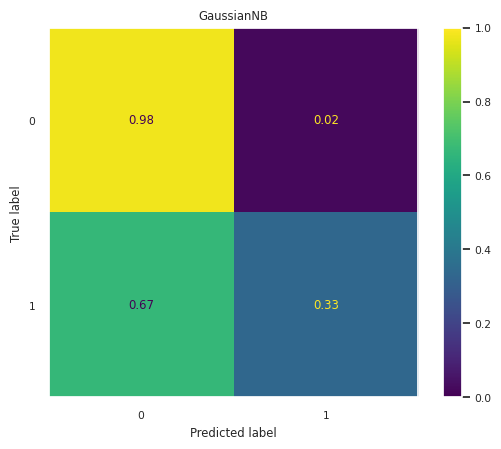
\includegraphics[width=\textwidth]{images/models/GNB_base.png}
        \caption{Baseline}
        %\label{fig:Ada_base}
    \end{subfigure}
    \begin{subfigure}[c]{0.4\textwidth}
        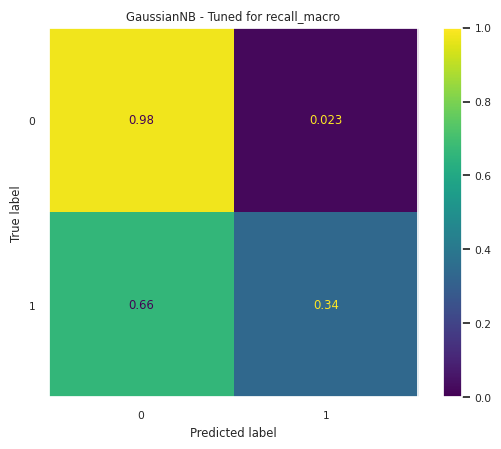
\includegraphics[width=\textwidth]{images/models/GNB_tuned.png}
        \caption{Tuned}
        %\label{fig:Ada_tuned}
    \end{subfigure}
    \caption{\subsecname\ results}
    %\label{fig:Ada_results}
\end{figure}
\end{frame}

\subsection{Perceptron}
\begin{frame}{\subsecname}
\begin{columns}
    \column{0.5\textwidth}
    \begin{table}
        \footnotesize
        \centering
        \begin{tabular}{ll}
            parameter & tuned value \\
            \hline\hline
            \txt{early_stopping} & \txt{True} \\
            \txt{penalty} & \txt{None} \\
            \txt{class_weight} & \txt{"balanced"} \\
            \txt{eta0} & 1.0 \\
        \end{tabular}
        %\label{tab:my_label}
    \end{table}
    \column{0.5\textwidth}
    \begin{table}
        \footnotesize
        \centering
        \begin{tabular}{lc}
            metric & result \\
            \hline\hline
            \txt{recall} (class 1) & 72\% \\
            \txt{recall_macro} & 79\% \\
        \end{tabular}
        %\label{tab:my_label}
    \end{table}
\end{columns}

\begin{figure}
    \centering
    \begin{subfigure}[c]{0.4\textwidth}
        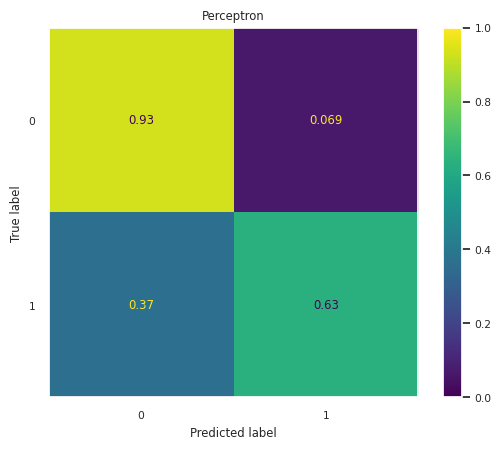
\includegraphics[width=\textwidth]{images/models/Percep_base.png}
        \caption{Baseline}
        %\label{fig:Ada_base}
    \end{subfigure}
    \begin{subfigure}[c]{0.4\textwidth}
        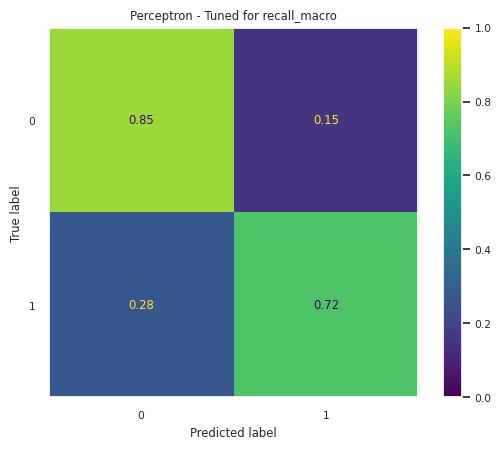
\includegraphics[width=\textwidth]{images/models/Percep_tuned.png}
        \caption{Tuned}
        %\label{fig:Ada_tuned}
    \end{subfigure}
    \caption{\subsecname\ results}
    %\label{fig:Ada_results}
\end{figure}
\end{frame}

\subsection{Support Vector Machine}
\begin{frame}{\subsecname}
\begin{columns}
    \column{0.5\textwidth}
    \begin{table}
        \scriptsize
        \centering
        \begin{tabular}{ll}
            parameter & tuned value \\
            \hline\hline
            \txt{kernel} & \txt{"poly"} \\
            \txt{class_weight} & \txt{"balanced"} \\
            \txt{shrinking} & \txt{False} \\
            \txt{gamma} & \txt{"auto"} \\
            \txt{C} & \txt{100} \\
        \end{tabular}
        %\label{tab:my_label}
    \end{table}
    \column{0.5\textwidth}
    \begin{table}
        \footnotesize
        \centering
        \begin{tabular}{lc}
            metric & result \\
            \hline\hline
            \txt{recall} (class 1) & 85\% \\
            \txt{recall_macro} & 88\% \\
        \end{tabular}
        %\label{tab:my_label}
    \end{table}
\end{columns}

\begin{figure}
    \centering
    \begin{subfigure}[c]{0.32\textwidth}
        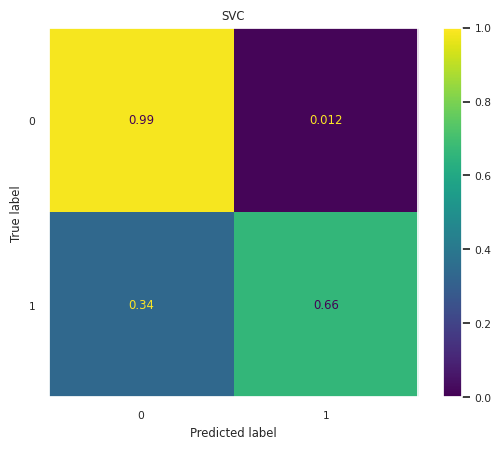
\includegraphics[width=\textwidth]{images/models/SVM_base.png}
        \caption{Baseline}
        %\label{fig:Ada_base}
    \end{subfigure}
    \begin{subfigure}[c]{0.32\textwidth}
        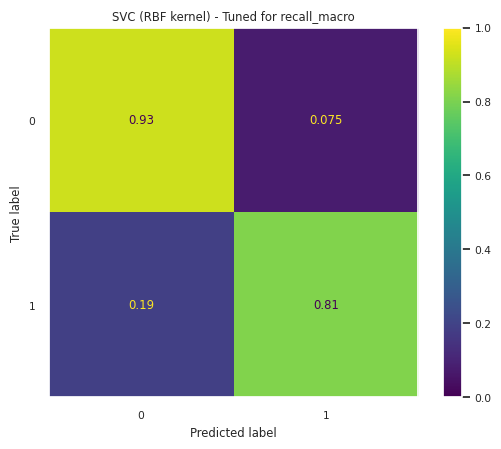
\includegraphics[width=\textwidth]{images/models/SVM_tuned_rbf.png}
        \caption{Tuned (RBF)}
        %\label{fig:Ada_tuned}
    \end{subfigure}
    \begin{subfigure}[c]{0.32\textwidth}
        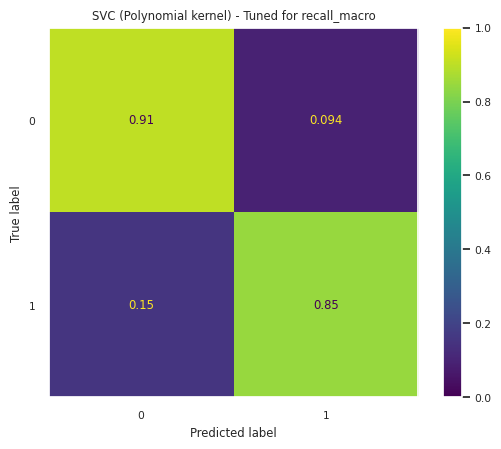
\includegraphics[width=\textwidth]{images/models/SVM_tuned_poly.png}
        \caption{Tuned (Polynomial)}
        %\label{fig:Ada_tuned}
    \end{subfigure}
    \caption{\subsecname\ results}
    %\label{fig:Ada_results}
\end{figure}
\end{frame}

\subsection{Gradient Descent}
\begin{frame}{\subsecname}
\begin{columns}
    \column{0.5\textwidth}
    \begin{table}
        \scriptsize
        \centering
        \begin{tabular}{ll}
            parameter & tuned value \\
            \hline\hline
            \txt{class_weight} & \txt{"balanced"} \\
            \txt{penalty} & \txt{"elasticnet"} \\
            \txt{learning_rate} & \txt{"invscaling"} \\
            \txt{loss} & \txt{"hinge"} \\
            \txt{alpha} & 1.0 \\
            \txt{eta0} & 0.1 \\
        \end{tabular}
        %\label{tab:my_label}
    \end{table}
    \column{0.5\textwidth}
    \begin{table}
        \footnotesize
        \centering
        \begin{tabular}{lc}
            metric & result \\
            \hline\hline
            \txt{recall} (class 1) & 80\% \\
            \txt{recall_macro} & 80\% \\
        \end{tabular}
        %\label{tab:my_label}
    \end{table}
\end{columns}
\vspace{-1.0em}
\begin{figure}
    \centering
    \begin{subfigure}[c]{0.4\textwidth}
        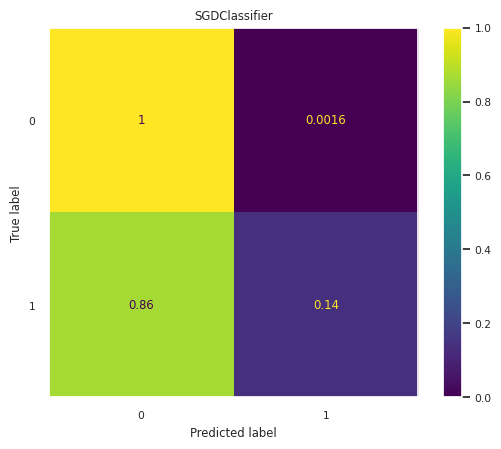
\includegraphics[width=\textwidth]{images/models/SGD_base.png}
        \caption{Baseline}
        %\label{fig:Ada_base}
    \end{subfigure}
    \begin{subfigure}[c]{0.4\textwidth}
        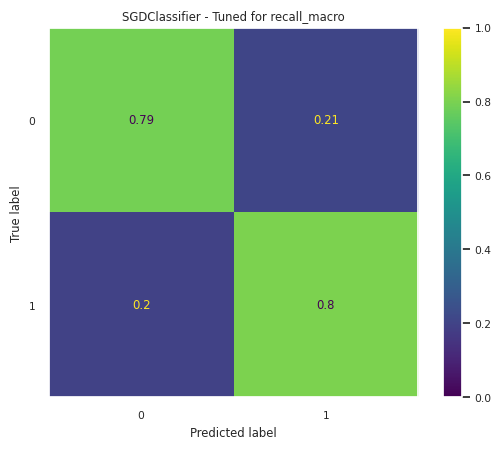
\includegraphics[width=\textwidth]{images/models/SGD_tuned.png}
        \caption{Tuned}
        %\label{fig:Ada_tuned}
    \end{subfigure}
    \caption{\subsecname\ results}
    %\label{fig:Ada_results}
\end{figure}
\end{frame}

\section{RESULTS}
\begin{frame}{\secname}
\end{frame}

\subsection{Model performances}
\begin{frame}{\subsecname}
After tuning, the models can be ranked as follows:

\begin{table}
    \centering
    \begin{tabular}{l|cc}
         & Class 1 recall & Recall macro average \\
         \hline\hline
         \textbf{Random Forest} & 84\% & \textbf{89\%} \\
         \textbf{SVM} & \textbf{85\%} & 88\% \\
         SGD & 80\% & 80\% \\
         Perceptron & 72\% & 79\% \\
         Decision Tree & 71\% & 83\% \\
         AdaBoost & 55\% & 77\% \\
         KNN & 45\% & 72\% \\
         Gaussian NB & 34\% & 66\% \\
    \end{tabular}
    \label{tab:my_label}
\end{table}

We therefore see that the Random Forest and SVM models can both be considered the most performant. However, being a few orders of magnitude faster to train, the former may be considered more optimal.

\end{frame}

\begin{frame}{\subsecname}
\begin{figure}
    \centering
    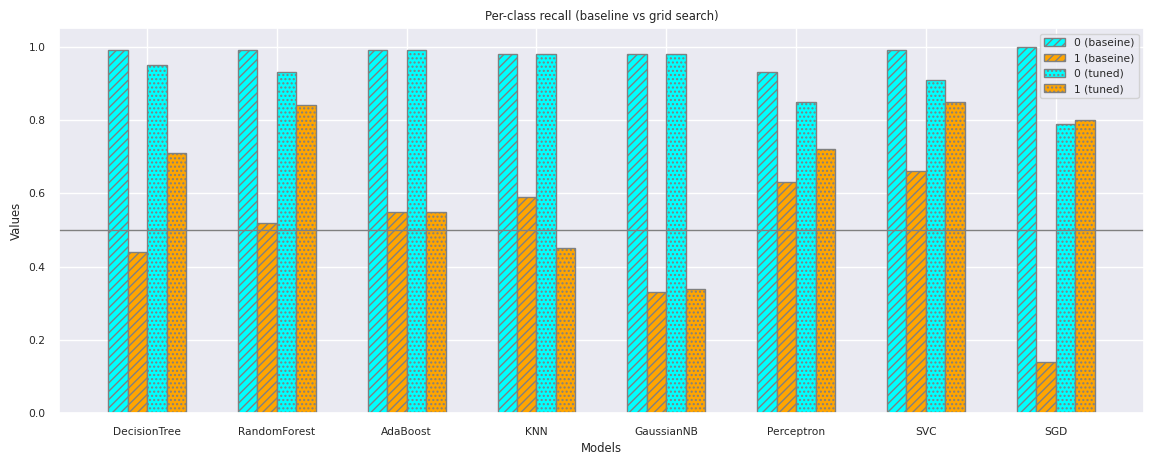
\includegraphics[width=1\linewidth]{images/recalls_before_after.png}
    \caption{Class recall before and after tuning}
    \label{fig:recall_before_after}
\end{figure}
\end{frame}

\begin{frame}{\subsecname}
\begin{figure}
    \centering
    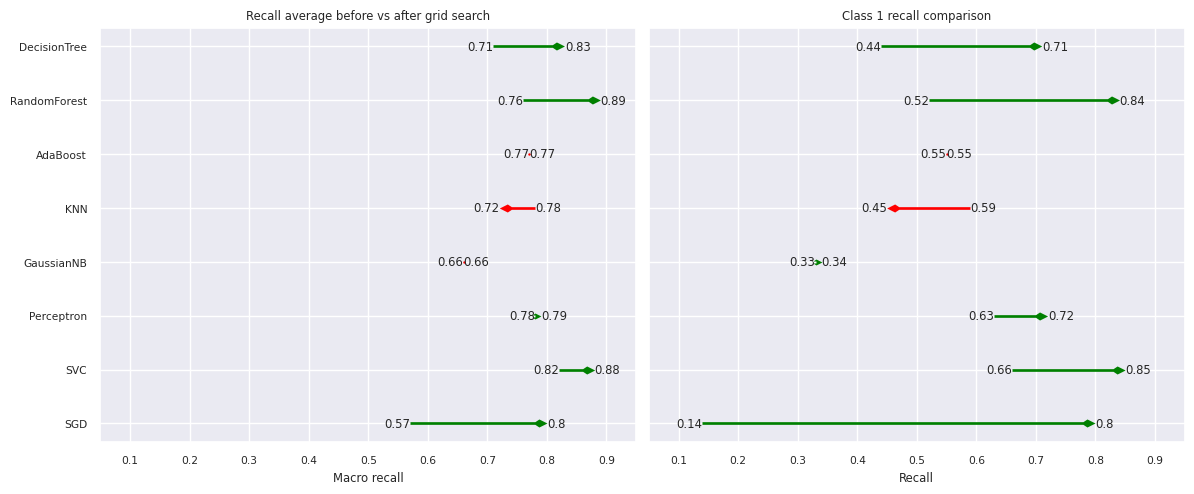
\includegraphics[width=1\linewidth]{images/recall_change.png}
    \caption{Class 1 recall and \txt{recall_macro} change with tuning}
    \label{fig:recall_change}
\end{figure}
\end{frame}

\subsection{Conclusions}
\begin{frame}{\subsecname}
The particularly bad performance of the KNN and Gaussian Naive Bayes classifiers was, to be fair, expected, though for different reasons:
\begin{itemize}
    \small
    \justifying
    \item For the former, the plots in figure \ref{fig:pairplots} show that the two classes are mostly overlapping and to not form well distinct clusters
    \item For the latter, its basic assumption of conditional independence between the attributes is clearly faulty in this context, since (for example) the rotational speed of a machine obviously influences its operating temperature
\end{itemize}

Furthermore, figure \ref{fig:recall_change} shows that these two models, and AdaBoost, either didn't improve or became worse. This may have two reasons:
\begin{itemize}
    \small
    \justifying
    \item none have a "class weight" parameter, and thus couldn't be tuned to "pay more attention" to one class than the other
    \item cross-validation is performed on a \textit{slice} of the training set (unlike the default model, which used all of it). This is especially damning for the KNN classifier because it doesn't really perform any analysis of the training data, instead simply using it "as-is".
\end{itemize}

\end{frame}

\begin{frame}{\subsecname}
The main focus of this project ended up being \textit{how to deal with severely imbalanced data}, more than a classification task itself. This, at least for the given dataset, was achieved in three main ways:
\begin{enumerate}
    \justifying
    \small
    \item using a per-class weighing of the datapoints, when supported
    \item performing dataset resampling during preprocessing to make the minority class easier to learn
    \item targeting the \txt{recall_macro} scoring metric when tuning instead of accuracy or precision
    \begin{itemize}
        \item this metric is an \textit{unweighted} average of the recalls for each class, making thus sure that the result doesn't de-facto only account for the majority datapoints
        \item the majority class being so dominant, it is acceptable to be slightly less accurate in classifying it if it means being way more sensitive to the minority
    \end{itemize}
\end{enumerate}

\end{frame}

\begin{frame}[allowframebreaks]{References}
    \small
    \bibliography{bibliography}
\end{frame}

\end{document}